% Based on docs/ambiguities/template.tex.
% Build from repository root: make questions LECTURE=06
\documentclass[a4paper,12pt]{article}
\usepackage[margin=19mm]{geometry}
\usepackage{amsmath,amssymb,graphicx,xcolor}
\usepackage{fontspec}
\usepackage{xepersian}
\settextfont{XB Roya}
\setlatintextfont{Latin Modern Roman}
\definecolor{ink}{HTML}{173D75}
\graphicspath{{images/}}
\setlength{\parindent}{0pt}
\setlength{\parskip}{5pt}
\linespread{1.12}
\newcommand{\qtitle}[2]{{\Large\bfseries\color{ink} پرسش \lr{#1}: #2}\par}
\newcommand{\answer}{\vfill\textbf{پاسخ یا صورت مورد تأیید و تاریخ:}\par\vspace{22mm}\hrule\medskip}
\newcommand{\sourcefile}{\begin{LTR}\small\texttt{sources/lectures/06 simple and semisimple modules.pdf}\end{LTR}}
\begin{document}
{\LARGE\bfseries پرسش‌های ابهام جلسهٔ ۰۶}\par
{\large مدول‌های ساده و نیمه‌ساده؛ جزوهٔ جبر پیشرفتهٔ دکتر خسروی}\par
شمارهٔ صفحه‌ها، شمارهٔ یک‌مبنای صفحه در فایل پی‌دی‌اف است، نه شمارهٔ دست‌نویس.
این دو پرسش هنوز حل نشده‌اند؛ ادعاهای وابسته به آن‌ها در اسلایدها قطعی نیستند.
\medskip\hrule\medskip

\qtitle{L06-Q01}{حلقهٔ ضرایب در مثال نقض}
\textbf{وضعیت:} در انتظار پاسخ؛ هنوز پاسخی ثبت نشده است.\par
\textbf{نشانی منبع:} نسخهٔ \lr{primary}، صفحهٔ ۳، مثال نقض با قلم قرمز؛ به‌ویژه فرمول نخست.
\sourcefile
\textbf{عبارت منبع:}
\[
 S=R[x]/\langle x^2\rangle.
\]
در متن آمده است که \(S/\langle x\rangle\) و \(\langle x\rangle\)
دو \(S\)-مدول ساده‌اند، ولی \(S\) نیمه‌ساده نیست و
\(\langle x\rangle\) تنها زیرمدول ماکسیمال آن است.
\begin{center}
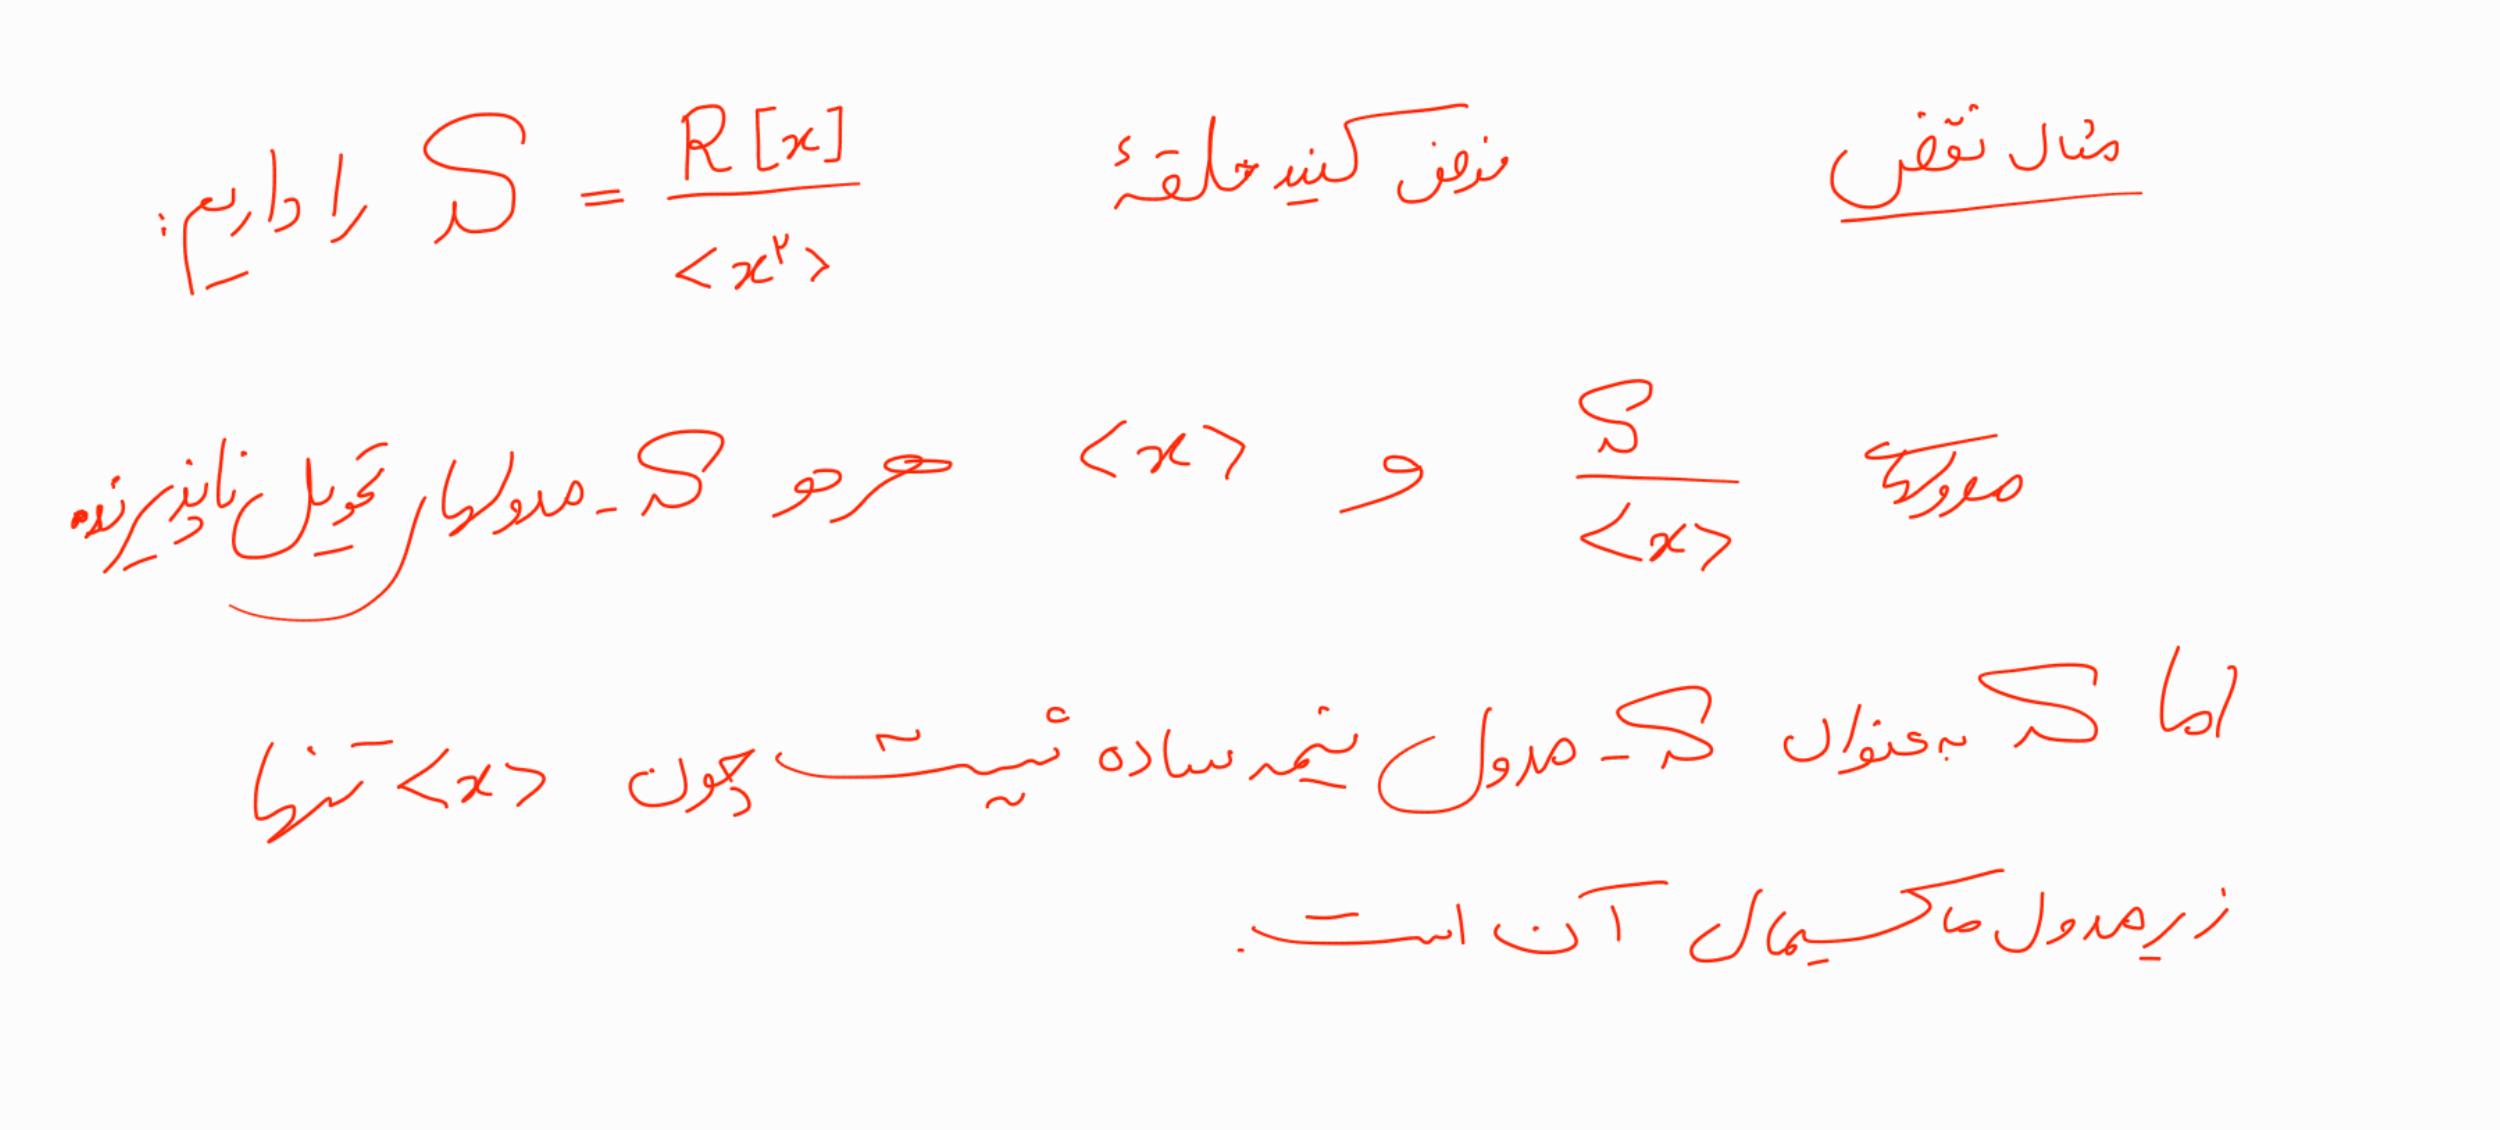
\includegraphics[width=\linewidth,height=57mm,keepaspectratio]{coefficient-ring.png}
\end{center}
\textbf{خوانش‌های ممکن:} \(R\) نماد میدان اعداد حقیقی \(\mathbb R\) است؛
یا میدان یا حلقهٔ تقسیم بودن آن به‌طور ضمنی فرض شده است؛ یا همان حلقهٔ دلخواهِ بحث است.

\textbf{دلیل پرسش:} ساده بودن دو مدول و ادعای یکتایی زیرمدول ماکسیمال
برای یک حلقهٔ ضرایب دلخواه برقرار نیست. در صفحات مجاور نیز فرضی برای \(R\) در این مثال دیده نمی‌شود.

\textbf{پرسش:} در این مثال، منظور از \(R\) چیست؟
آیا \(R=\mathbb R\) است، یا باید فرض کنیم \(R\) میدان یا حلقهٔ تقسیم است؟
اگر حلقهٔ دیگری منظور است، فرض دقیق آن را مشخص کنید.

\textbf{پس از پاسخ:} فرض تأییدشده در مثال اسلاید ثبت می‌شود و این پرسش
همراه پاسخ، نتیجهٔ ویرایش و تاریخ، در این پرونده و دفتر ثبت جلسه حفظ خواهد شد.
\answer
\newpage

{\large\bfseries پرسش‌های ابهام جلسهٔ ۰۶؛ ادامه}\par
\qtitle{L06-Q02}{برابری یا یکریختی در تجزیهٔ زیرمدول}
\textbf{وضعیت:} در انتظار پاسخ؛ هنوز پاسخی ثبت نشده است.\par
\textbf{نشانی منبع:} نسخهٔ \lr{primary}، پایین صفحهٔ ۴، صورت قضیه؛
میانهٔ بالایی صفحهٔ ۵، نتیجهٔ اثبات.
\sourcefile
\textbf{صورتِ نوشته‌شده:} اگر \(M=\sum_{i\in I}M_i\) و \(M_i\)ها
زیرمدول‌های سادهٔ \(M\) باشند، برای هر \(N\leqslant M\)، زیرمجموعهٔ
\(J\subseteq I\) وجود دارد که \(N=\bigoplus_{j\in J}M_j\).
\begin{center}
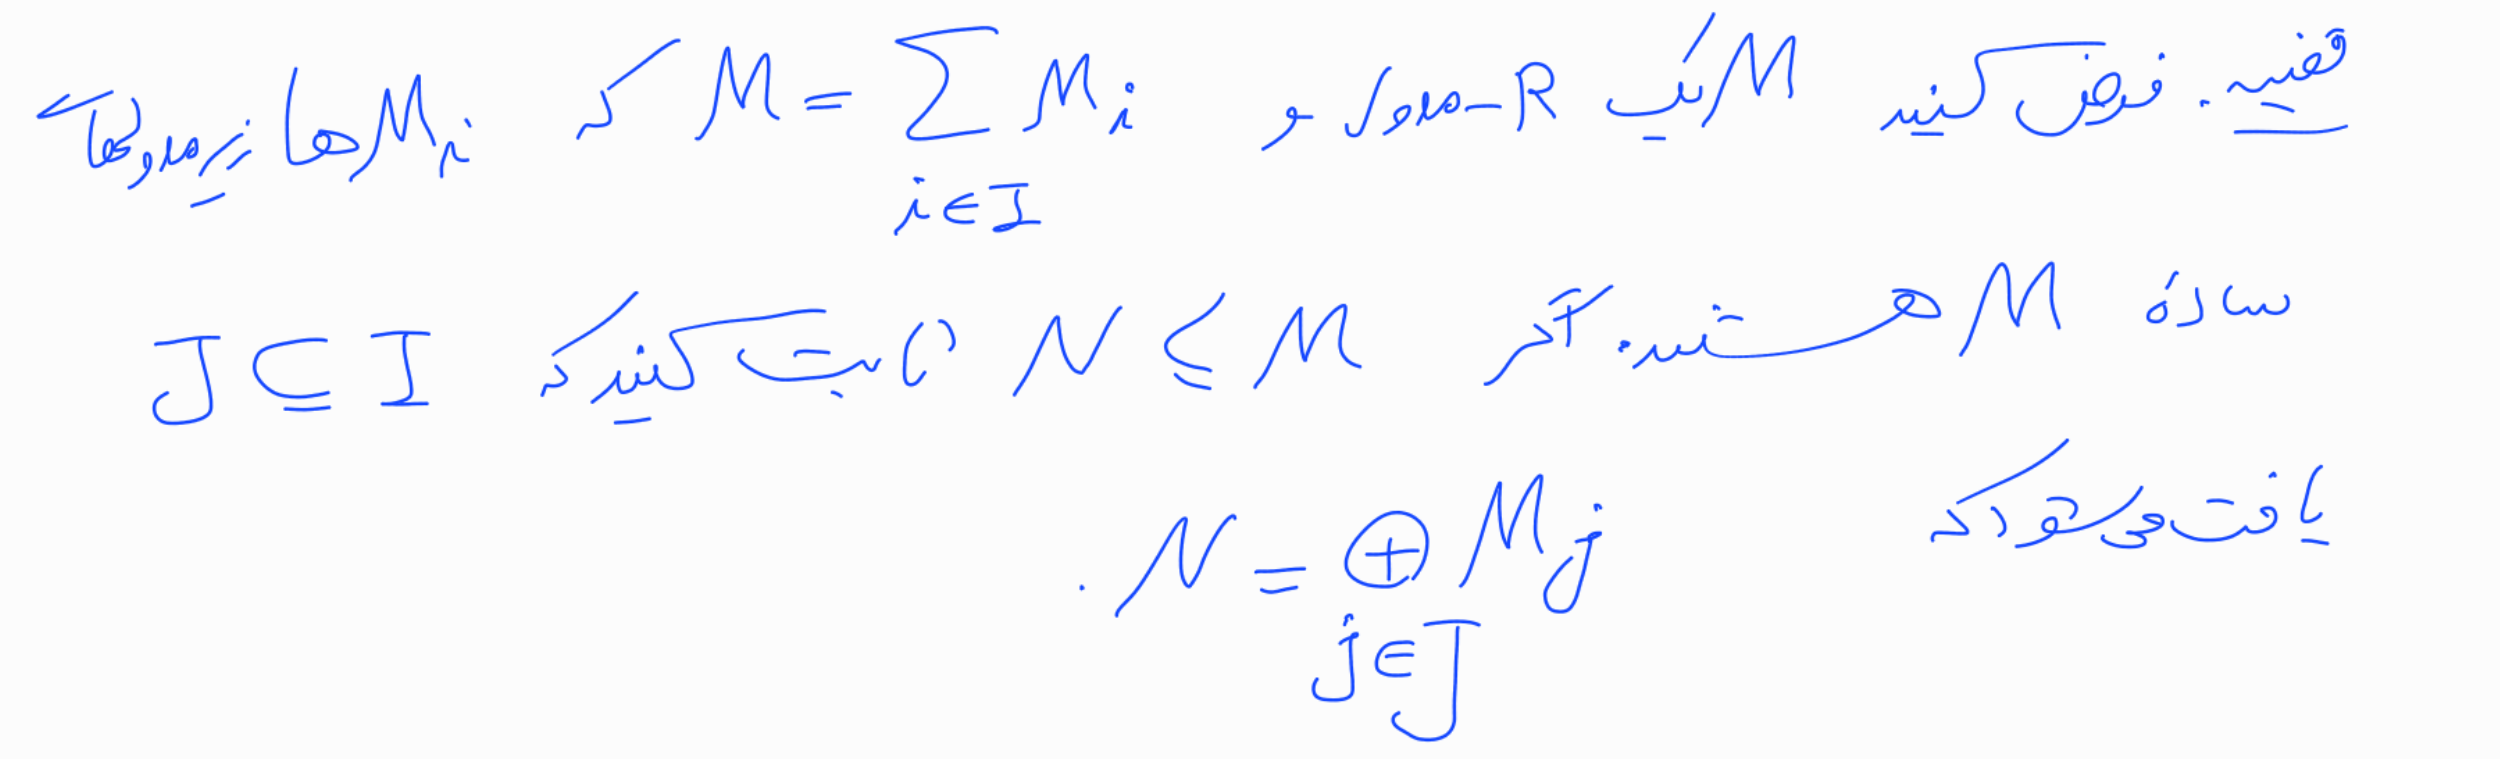
\includegraphics[width=\linewidth,height=42mm,keepaspectratio]{submodule-statement.png}\\[-1pt]
{\small صورت قضیه در صفحهٔ ۴}
\end{center}
\textbf{نتیجهٔ اثبات در صفحهٔ ۵:}
\[
 N\cong M\Big/\left(\bigoplus_{i\in J_1}M_i\right)
   \cong\bigoplus_{i\in J_0\setminus J_1}M_i.
\]
\begin{center}
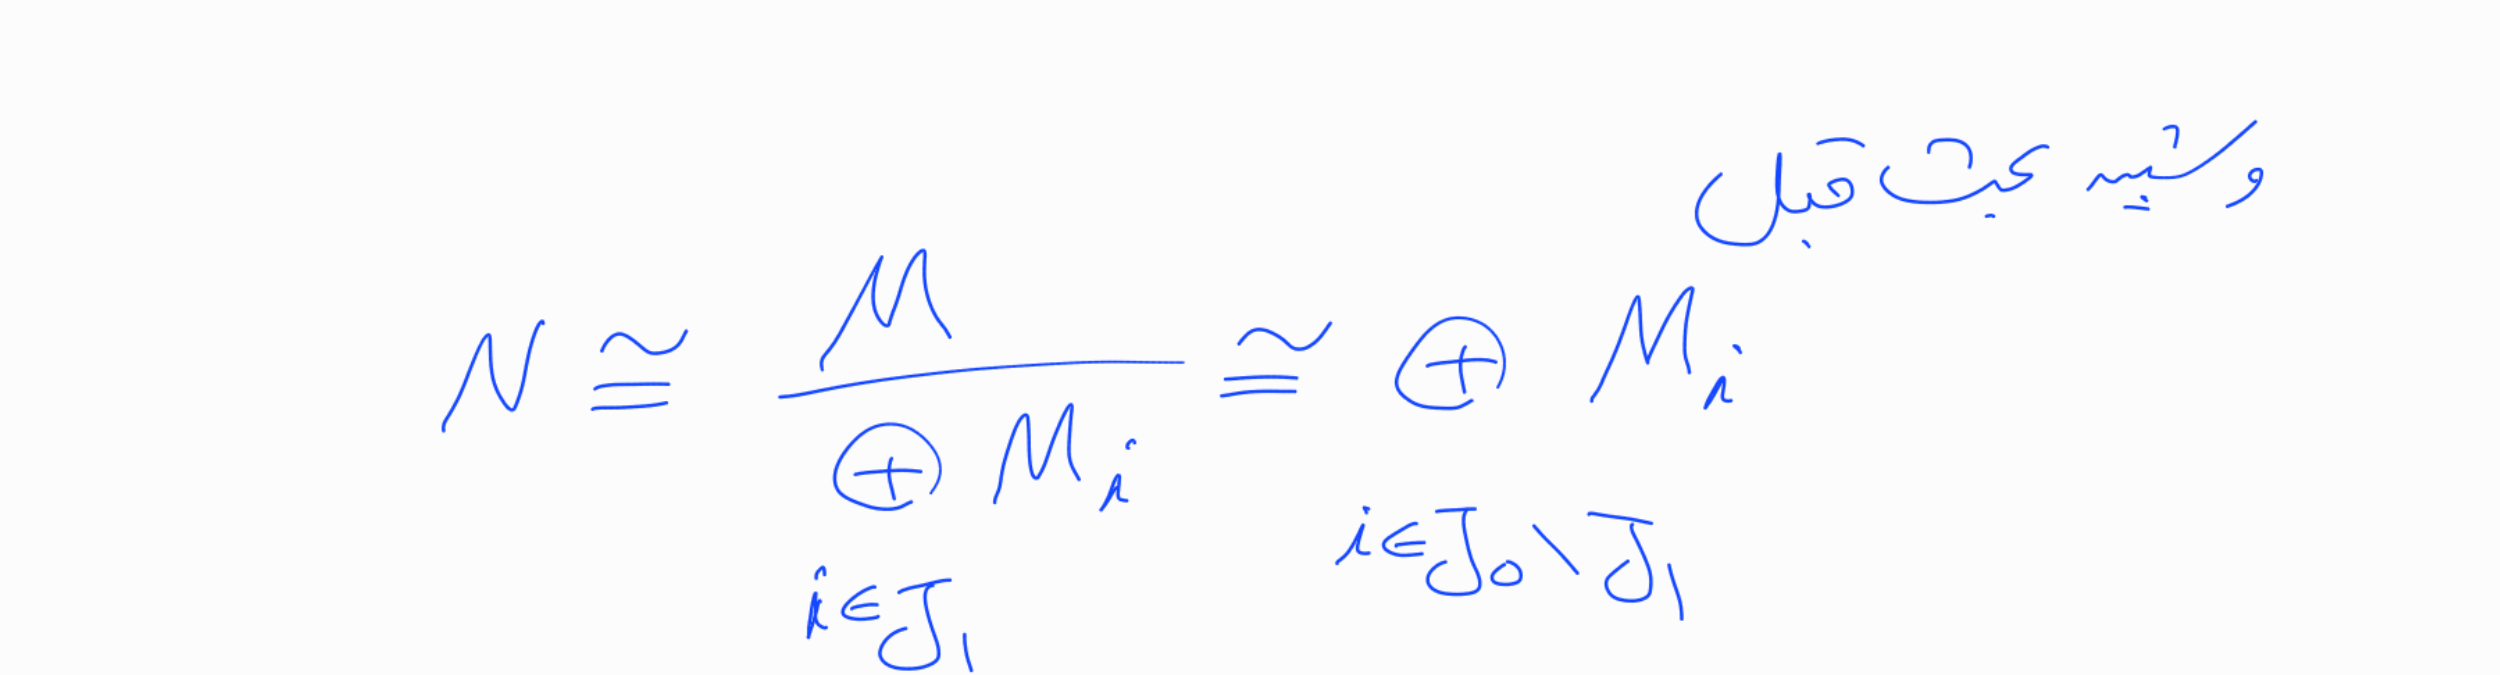
\includegraphics[width=\linewidth,height=33mm,keepaspectratio]{submodule-proof.png}\\[-1pt]
{\small یکریختی‌های پایان اثبات در صفحهٔ ۵}
\end{center}
\textbf{خوانش‌های ممکن و اثر تفاوت:} برابری با جمعِ زیرخانواده‌ای از
همان زیرمدول‌های داده‌شده، از یکریختی با آن جمع قوی‌تر است؛
اثبات فقط یکریختی را نتیجه می‌دهد. برابری برای یک زیرمدول دلخواه لزوماً برقرار نیست.

\textbf{پرسش:} آیا در صورت قضیه، مطابق اثبات، به‌جای برابری بنویسم
\(N\cong\bigoplus_{j\in J}M_j\)؟
اگر برابری مقصود است، فرض تکمیلی یا صورت دقیق مورد تأیید را مشخص کنید.

\textbf{پس از پاسخ:} صورت تأییدشده در اسلاید ثبت می‌شود و پاسخ، نتیجهٔ ویرایش
و تاریخ در این پرونده و دفتر ثبت جلسه حفظ خواهد شد.
\answer
\end{document}
